\documentclass[notheorems,serif,table,compress]{beamer}  %dvipdfm选项是关键,否则编译统统通不过
%%------------------------常用宏包------------------------
%%注意, beamer 会默认使用下列宏包: amsthm, graphicx, hyperref, color, xcolor, 等等
\usepackage{fontspec,xunicode,xltxtra}  % for XeTeX
\usepackage{verbatim}
%\usepackage{mathabx}
\usepackage{latexsym}
\usepackage{amsfonts,amssymb}
\usepackage{styles/iplouclistings}
\usepackage{fancybox}
\usepackage{colortbl}
\usepackage{tcolorbox}
%\usepackage[T1]{fontenc}
%\usepackage{bookman}
\usepackage{subfigure}
\usepackage{hyperref}
\usepackage{listings}
\usepackage{animate}
\usepackage[absolute,overlay]{textpos}
\usepackage{graphicx}
\usepackage{tikz}
\usepackage[americaninductors,europeanresistors]{circuitikz}
\usepackage{tikz}
\usepackage{fancybox}     %% 定义zhushadow时用到
\usepackage{pifont} %ding用到
\newsavebox{\mysaveboxOne}  %%为了在only中使用lstlisting
\newsavebox{\mysaveboxTwo}
\newsavebox{\mysaveboxThree}
\newsavebox{\mysaveboxFour}
\newsavebox{\mysaveboxFive}
\newsavebox{\mysaveboxSix}
\newsavebox{\mysaveboxSeven}
\newcommand\zhushadow[2][purple]{\hskip5pt\shadowbox{\color{#1}\small\kai #2\vspace{3mm}}}

%%------------------------ThemeColorFont------------------------
%% Presentation Themes
% \usetheme[<options>]{<name list>}
%\usetheme{Madrid}
\usetheme{Berkeley}
%% Inner Themes双精度计算
% \useinnertheme[<options>]{<name>}
%% Outer Themes
% \useoutertheme[<options>]{<name>}
%\useoutertheme{miniframes} 
%% Color Themes 
%\usecolortheme[<options>]{<name list>}
%% Font Themes
\usefonttheme{serif}
\setbeamertemplate{background canvas}[vertical shading][bottom=white,top=structure.fg!7] %%背景色, 上25%的蓝, 过渡到下白.
\setbeamertemplate{theorems}[numbered]
\setbeamertemplate{navigation symbols}{}   %% 去掉页面下方默认的导航条.
\usepackage{styles/zhfontcfg}
%\setsansfont[Mapping=tex-text]{文泉驿正黑}  %% 需要fontspec宏包
     %如果装了Adobe Acrobat,可在font.conf中配置Adobe字体的路径以使用其中文字体
     %也可直接使用系统中的中文字体如SimSun,SimHei,微软雅黑 等
     %原来beamer用的字体是sans family;注意Mapping的大小写,不能写错
     %设置字体时也可以直接用字体名,以下三种方式等同:
     %\setromanfont[BoldFont={黑体}]{宋体}
     %\setromanfont[BoldFont={SimHei}]{SimSun}
     %\setromanfont[BoldFont={"[simhei.ttf]"}]{"[simsun.ttc]"}
%%------------------------MISC------------------------
\graphicspath{{figures/}}         %% 图片路径. 本文的图片都放在这个文件夹里了.
%%------------------------listing------------------------
%\lstset{language=[LaTeX]TeX,Python}
%%------------------------正文------------------------
\begin{document}
\XeTeXlinebreaklocale "zh"         % 表示用中文的断行
\XeTeXlinebreakskip = 0pt plus 1pt % 多一点调整的空间
%%----------------------------------------------------------
%% This is only inserted into the PDF information catalog. Can be left
%% out.
%%%
%% Delete this, if you do not want the table of contents to pop up at
%% the beginning of each subsection:
%\AtBeginSection[]{                              % 在每个Section前都会加入的Frame
%  \frame<handout:0>{
%    \frametitle{Contents}\small
%    \tableofcontents[current,currentsubsection]
%  }
%}
%
%\AtBeginSubsection[]                            % 在每个子段落之前
%{
%  \frame<handout:0>                             % handout:0 表示只在手稿中出现
%  {
%    \frametitle{Contents}\small
%    \tableofcontents[current,currentsubsection] % 显示在目录中加亮的当前章节
%  }
%}

\setbeamertemplate{caption}{\raggedright\insertcaption\par}

%%----------------------------------------------------------
\logo{
\includegraphics[scale=0.13]{ouclogo.png}}
\title{Image Interpolation}
%\subtitle{Bottom-Up Saliency Detection Model Based on Human Visual Sensitivity and Amplitude Spectrum}
\subtitle{图像内插}
\author[]{\textcolor{black}{丁昊}}
\institute[CVBIOUC]
{
\small\textcolor{violet}{CVBIOUC\\
%Ocean University of China\\
\url{http://vision.ouc.edu.cn/~zhenghaiyong}}
}
%\date[]{}
%\titlegraphic{
%\includegraphics[height=1.0cm]{ouc-logo.jpg}}
\frame{ \titlepage }
%%----------------------------------------------------------
%\section*{Contents}
\frame{\frametitle{目录}\tableofcontents}
%%----------------------------------------------------------
\def\hilite<#1>{\temporal<#1>{\color{blue!15}}{\color{black}}{\color{black}}}
\newcommand{\shadow}[2][purple]{\hskip5pt\shadowbox{\color{#1}\small \kai #2\vspace{3mm}}}
\newcommand{\colorrbox}[2][purple]{\doublebox{\color{#1}\small \kai#2}}

%============================================================================

\section{基本概念}

\subsection{简介}
\begin{frame}[fragile]
\frametitle{简介}
    内插是一个通过已知的离散数据求未知数据的过程。

    内插可以完成的功能:	
	\begin{itemize}
	\item 缩放图像
	\item 旋转图像
	\item 几何矫正
    	\end{itemize}
\end{frame}

\subsection{放大图像}
\begin{frame}
\frametitle{放大图像}
    放大图像(上采样upsamplin/图像插值interpolating)的主要目的是放大原图像,从而可以显示在更高分辨率的显示设备上。
\begin{figure}
        \begin{minipage}[t]{0.4\linewidth}
        \centering
        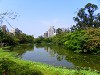
\includegraphics[width=0.3\linewidth]{template.png} 
        \end{minipage}
        \begin{minipage}[t]{0.4\linewidth}
        \centering
        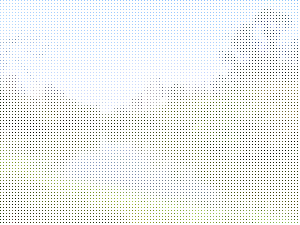
\includegraphics[width=1\linewidth]{template1.png} 
        \end{minipage}
    \end{figure}
%图像放大几乎都是采用内插值方法,即在原有图像像素的基础上在像素点之间采用合适的插值算法插入新的元素。
\end{frame}
 
\subsection{方法分类}

\begin{frame}
\frametitle{方法分类}
	\begin{cases}
	$传统插值算法$	
		\begin{cases}
		$最近邻插值$\\
		$双线性插值$\\
		$双三次插值$
		\end{cases}\\
	$基于边缘的图像插值算法$
		\begin{cases}
		$基于原始低分辨图像边缘$\\
		$基于插值后高分辨率图像边缘$
		\end{cases}\\
	$基于区域的图像插值算法$\\
	$其他方法$
	\end{cases}
\end{frame}


\section{最近邻插值}

\subsection{原理}
\begin{frame}
\frametitle{最近邻插值}
    	\begin{minipage}[t]{0.5\linewidth}
        \centering
        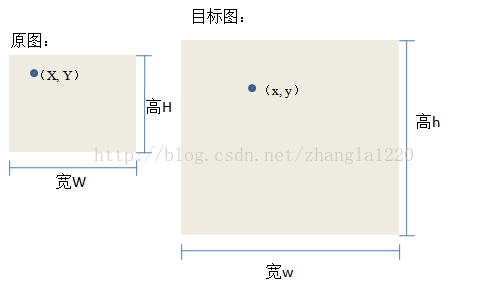
\includegraphics[width=1\linewidth]{near.jpg} 
        \end{minipage}
	\begin{minipage}[t]{0.4\linewidth}
        \centering
        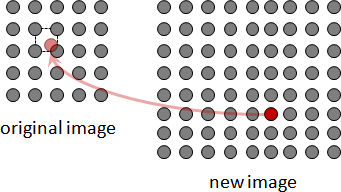
\includegraphics[width=1\linewidth]{n.png} 
        \end{minipage}
\end{frame}

\subsection{代码}
\begin{frame}
\frametitle{代码}
\href{code/nearest.cpp}{最近邻内插代码}
\end{frame}

\subsection{结果图}
\begin{frame}
\frametitle{结果图}
	\begin{minipage}[t]{0.4\linewidth}
        \centering
        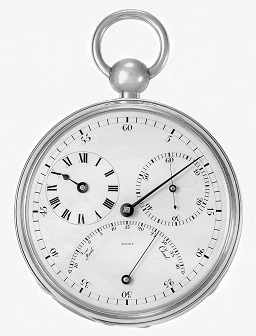
\includegraphics[width=0.5\linewidth]{1.jpg} 
        \end{minipage}
	\begin{minipage}[t]{0.4\linewidth}
        \centering
        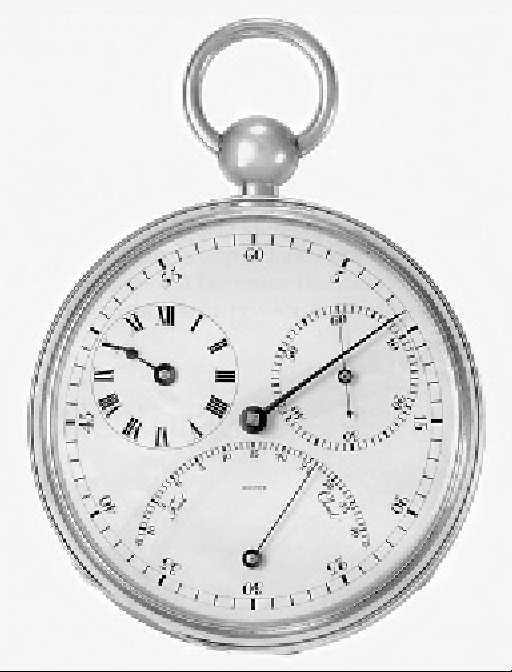
\includegraphics[width=1\linewidth]{nearest.jpg} 
        \end{minipage}

\end{frame}

\section{双线性插值}

\subsection{原理}
\begin{frame}
\frametitle{双线性插值}

1.$f(x,y) \approx f(0,0)(1-x)(1-y)+f(1,0)x(1-y)+f(0,1)(1-x)y+f(1,1)xy$

\mbox{}

2.
\begin{math}
v(x,y)=ax+by+cxy+d
\end{math}

\mbox{}

系数:
\begin{itemize}
\item a=f(1,0)-f(0,0)
\item b=f(0,1)-f(0,0)
\item c=f(1,1)-f(0,1)-f(1,0)+f(0,0)
\item d=f(0,0)
\end{itemize}
\end{frame}

\subsection{代码}
\begin{frame}
\frametitle{代码}
\href{code/bilinear.cpp}{双线性内插代码}
\end{frame}

\subsection{结果图}
\begin{frame}
\frametitle{结果图}
	\begin{minipage}[t]{0.4\linewidth}
        \centering
        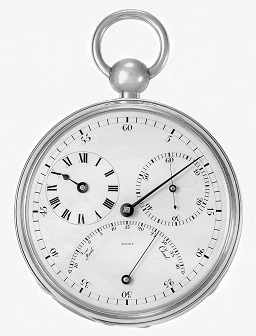
\includegraphics[width=0.5\linewidth]{1.jpg} 
        \end{minipage}
	\begin{minipage}[t]{0.4\linewidth}
        \centering
        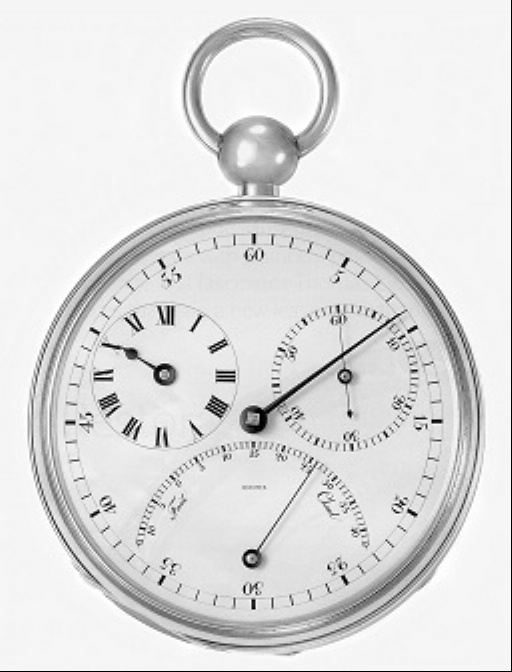
\includegraphics[width=1\linewidth]{Bilinear-pots.jpg} 
        \end{minipage}

\end{frame}
\section{双三次插值}

\subsection{原理}
\begin{frame}
\frametitle{双三次插值}
    	$f(x,y)=\sum _{i=0}^{3}\sum _{j=0}^{3}a_{ij}x^{i}y^{j}$

\mbox{}

计算系数 $a_{ij}$ 的取值依赖于插值数据的特性。一阶导数$f'x$与$f'y$ 表示x、y方向的表面斜率,二阶相互导数$f''xy$表示同时在x与y方向的斜率。

\mbox{}

对于网格单元的每个顶点,将局部坐标(0,0)、(1,0)、(0,1)和(1,1)带入这些方程,再解这16个方程。
\end{frame}

\subsection{代码}
\begin{frame}
\frametitle{代码}
\href{code/bicubic.cpp}{双三次内插代码}

\end{frame}

\subsection{结果图}
\begin{frame}
\frametitle{结果图}
	\begin{minipage}[t]{0.4\linewidth}
        \centering
        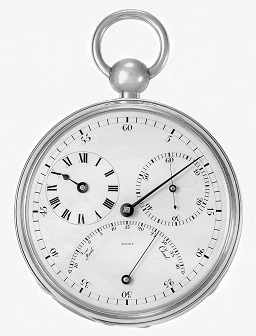
\includegraphics[width=0.5\linewidth]{1.jpg} 
        \end{minipage}
	\begin{minipage}[t]{0.4\linewidth}
        \centering
        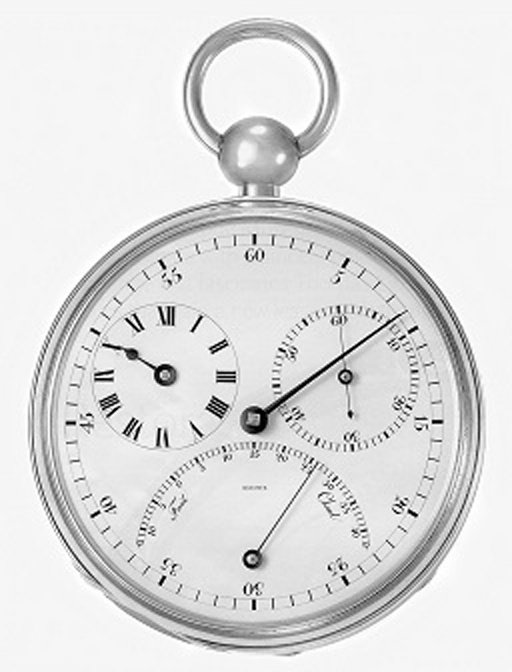
\includegraphics[width=1\linewidth]{Bicubic.jpg} 
        \end{minipage}
\end{frame}

\section{结论}

\subsection{对比图}

\begin{frame}
\frametitle{对比图}
	\begin{minipage}[t]{0.32\linewidth}
        \centering
        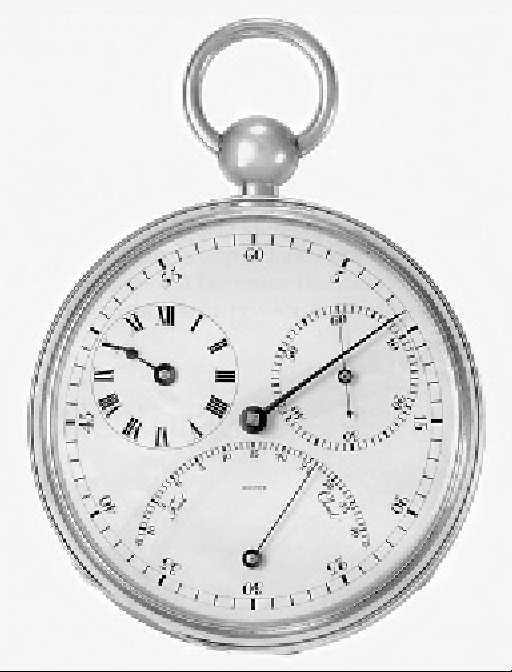
\includegraphics[width=0.9\linewidth]{nearest.jpg} 
        \end{minipage}
	\begin{minipage}[t]{0.32\linewidth}
        \centering
        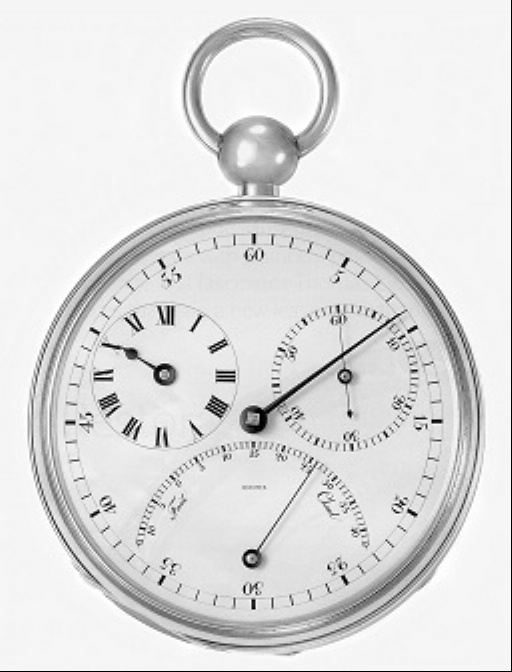
\includegraphics[width=0.9\linewidth]{Bilinear-pots.jpg} 
        \end{minipage}
	\begin{minipage}[t]{0.32\linewidth}
        \centering
        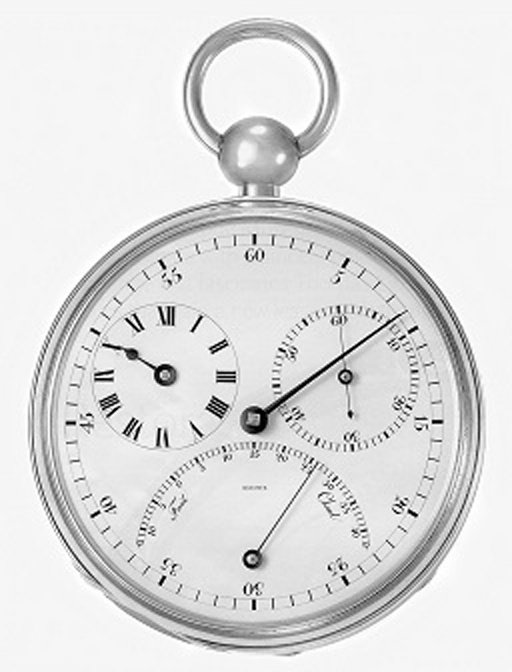
\includegraphics[width=0.9\linewidth]{Bicubic.jpg} 
        \end{minipage}
\end{frame}

\subsection{结论}
\begin{frame}
\frametitle{结论}
	\textbf{\color{blue}1. 图像还原度: }\\
	\mbox{}
	\begin{minipage}[t]{1\linewidth}
        \centering
        双三次内插 > 双线性内插 > 最近邻内插
        \end{minipage}
	\mbox{}
	\begin{minipage}[t]{1\linewidth}
	\textbf{\color{blue}2. 算法简易程度: }\\
	\end{minipage}
	\mbox{}
	\begin{minipage}[t]{1\linewidth}
        \centering
        最近邻内插 > 双线性内插 > 双三次内插
        \end{minipage}
	\mbox{}
	\begin{minipage}[t]{1\linewidth}
	\textbf{\color{red}$\rightarrow$ 双线性内插可满足大部分需求且不会过于复杂}
	\end{minipage}
\end{frame}

\end{document}
